%% LyX 1.1 created this file.  For more info, see http://www.lyx.org/.
%% Do not edit unless you really know what you are doing.
\documentclass[english]{article}
\usepackage[T1]{fontenc}
\usepackage[latin1]{inputenc}
% \usepackage{babel}
\usepackage{graphics}
\IfFileExists{url.sty}{\usepackage{url}}
                      {\newcommand{\url}{\texttt}}

\makeatletter

%%%%%%%%%%%%%%%%%%%%%%%%%%%%%% LyX specific LaTeX commands.
\providecommand{\LyX}{L\kern-.1667em\lower.25em\hbox{Y}\kern-.125emX\@}

%%%%%%%%%%%%%%%%%%%%%%%%%%%%%% Textclass specific LaTeX commands.
 \newenvironment{lyxlist}[1]
   {\begin{list}{}
     {\settowidth{\labelwidth}{#1}
      \setlength{\leftmargin}{\labelwidth}
      \addtolength{\leftmargin}{\labelsep}
      \renewcommand{\makelabel}[1]{##1\hfil}}}
   {\end{list}}
 \newenvironment{lyxcode}
   {\begin{list}{}{
     \setlength{\rightmargin}{\leftmargin}
     \raggedright
     \setlength{\itemsep}{0pt}
     \setlength{\parsep}{0pt}
     \normalfont\ttfamily}%
    \item[]}
   {\end{list}}
 \usepackage{verbatim}

%%%%%%%%%%%%%%%%%%%%%%%%%%%%%% User specified LaTeX commands.
\usepackage{dsfont}

% No date please
\date{}

\makeatother
\begin{document}
% This is for \LyX


\newcommand{\bfrac}[2]{\frac{#1 }{#2 }}



\newcommand{\nth}{^{\textrm{th}}}



\newcommand{\R}{R}



\newcommand{\N}{N}



\newcommand{\Z}{Z}



\newcommand{\tra}{^{T}}



\newcommand{\xx}{\mathbf{x}}


% This is for \LaTeX

\renewcommand{\R}{{\mathds{R}}} 

\renewcommand{\N}{{\mathds{N}}}

\renewcommand{\Z}{{\mathds{Z}}}

\renewcommand{\tra}{^{\top}}

\renewcommand{\bfrac}[2]{\frac{{\textstyle #1 }}{{\textstyle #2 }}}


\title{Mini-HOWTO : visualizing 3D data using Octave, VRML and FreeWRL%
\thanks{Author : Etienne Grossmann \texttt{<etienne@isr.ist.utl.pt>} (soon
replaced by {}``Octave-Forge developers''?). This document is free
documentation; you can redistribute it and/or modify it under the
terms of the GNU Free Documentation License as published by the Free
Software Foundation.\protect \\
.~~~This is distributed in the hope that it will be useful, but
WITHOUT ANY WARRANTY; without even the implied warranty of MERCHANTABILITY
or FITNESS FOR A PARTICULAR PURPOSE.
}}

\maketitle
\begin{comment}
Keywords: octave, tutorial, 3D visualization, VRML
\end{comment}
\begin{abstract}
This document shows how to visualize sets of 3D points, 3D curves,
surfaces etc using the numerical language Octave, in conjunction with
the VRML browser FreeWRL. The basic functionalities and principles
are presented here with examples, while the detailed synopsis can
be obtained from the online help system.
\end{abstract}
~
\begin{figure}
{\centering \resizebox*{0.38\textwidth}{!}{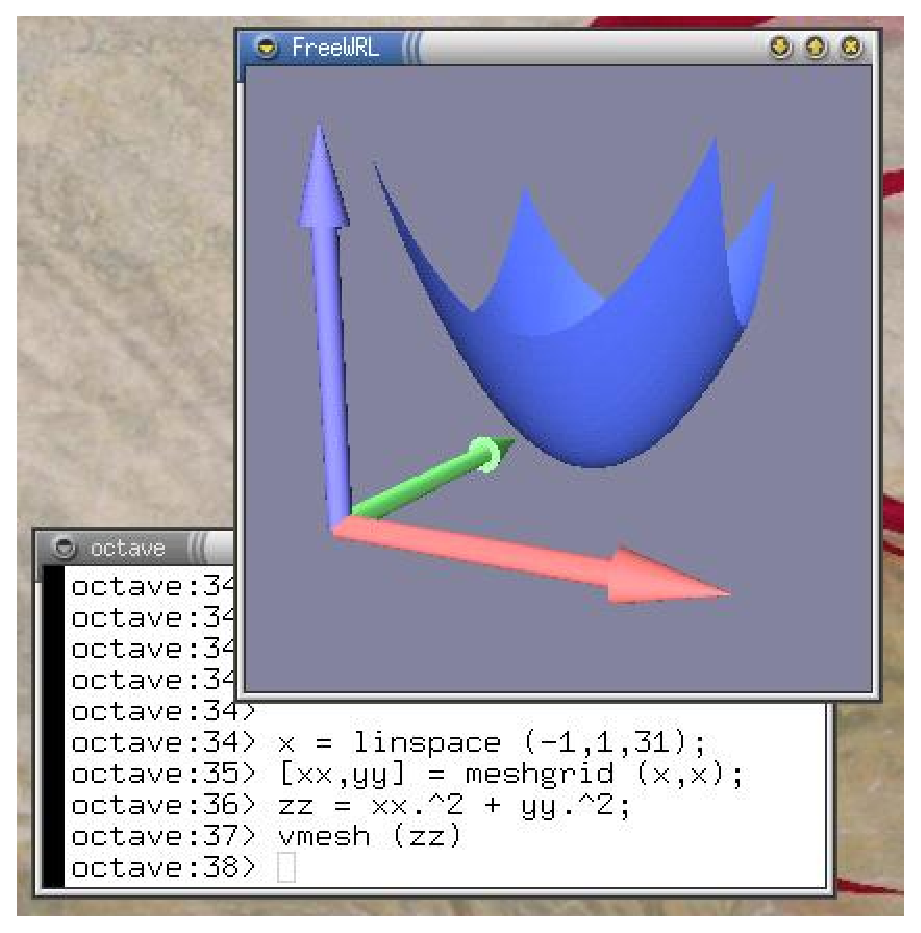
\includegraphics{figures/freewrl-octave-snap-2-c.eps}} ~\raisebox{5mm}{\resizebox*{0.55\textwidth}{!}{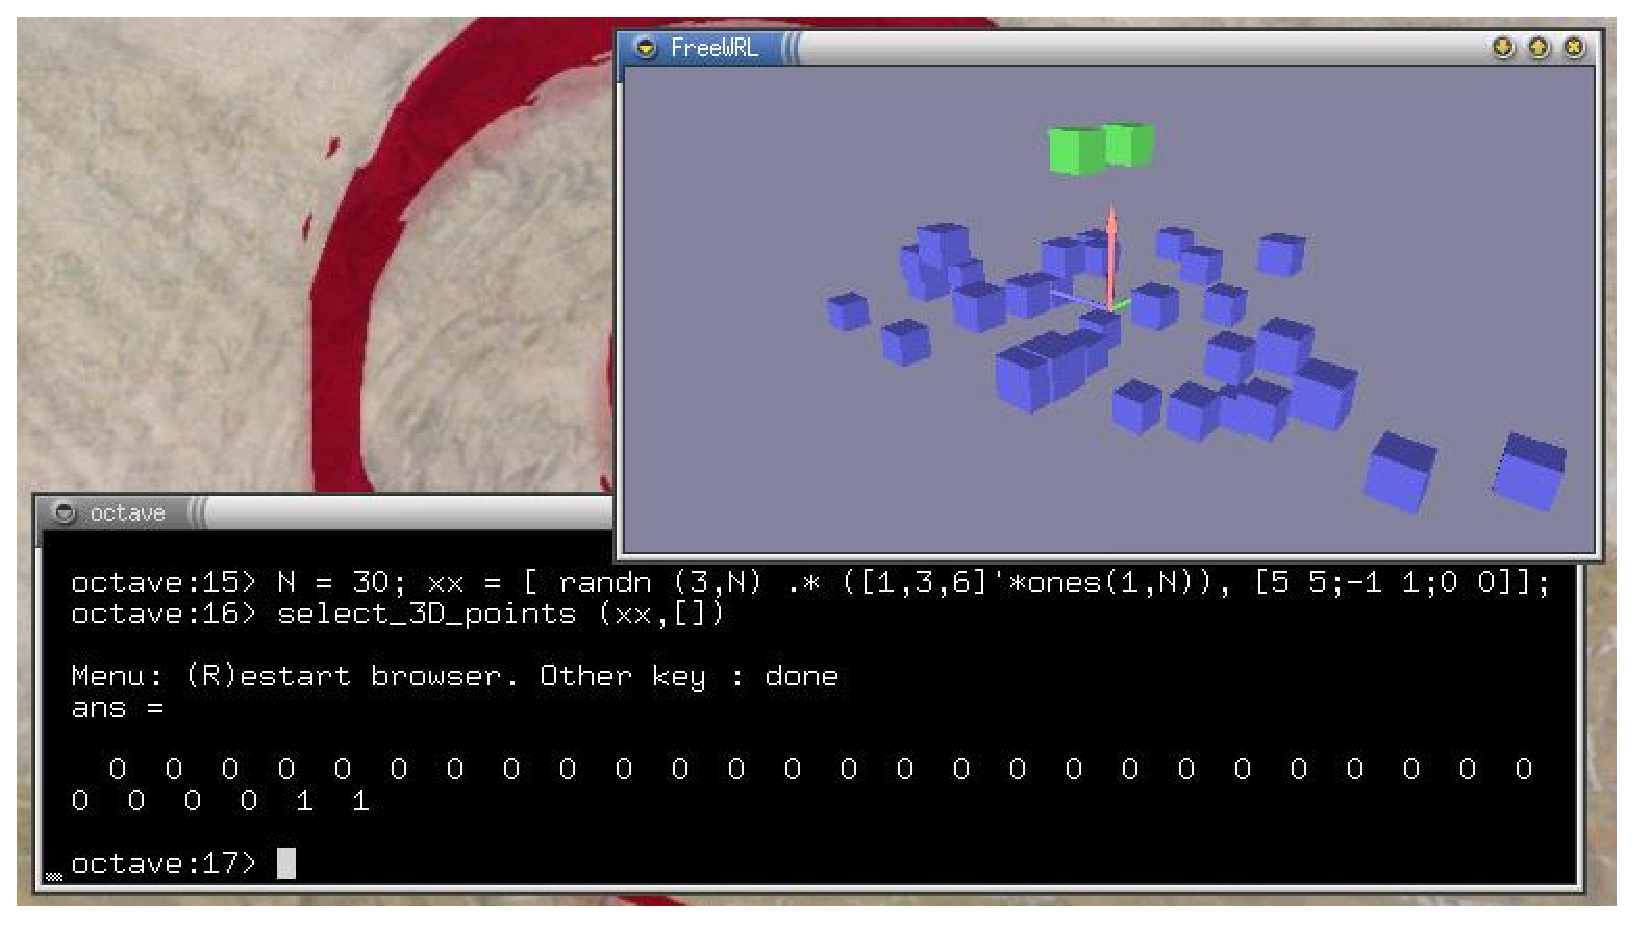
\includegraphics{figures/freewrl-select-points-2-c.eps}} }\par}


\caption{\label{fig:freewrloctave}FreeWRL window and octave running in a
terminal. The red and green vectors of the frame represent the {}``X''
and {}``Y'' axes. \textbf{Left:} Displaying the surface of a 2-variable
function. \textbf{Right:} Viewing a set of 3D points and selecting
a subset.}
\end{figure}
~


\paragraph{Prerequisites:}

It is assumed that you have installed Octave 2.1.35 (\url{http://www.octave.org})
or more, FreeWRL (\url{http://www.crc.ca/FreeWRL}) 0.34 or more (versions
between 0.27 and 0.31 may work too) and the Octave-Forge (\url{http://octave.sourceforge.net})
package. Each one is available from the indicated URL. Rudimentary
knowledge of Octave is also assumed.


\section{Basics\label{sec:basics}}

This document describes some 3D visualization functions from the Octave-Forge
package. First, examples are given on how to visualize a surface with
the \texttt{vmesh()} function and how to visualize a set of 3D points
and select a subset with the mouse. The basic usage of FreeWRL, the
program that does the 3D visualization are introduced at the same
time.

The second section explains more in detail how the VRML package works,
presents other functions and shows how to assemble various 3D objects.
Finally, a brief summary and plans for the future are given in Section~\ref{sec:conclusions}.


\subsection{Viewing a surface from the Octave prompt}

Consider the following Octave commands~:


\subparagraph{Listing 1}

\begin{lyxcode}
x~=~linspace~(-1,1,31);

{[}xx,yy{]}~=~meshgrid~(x,x);

zz~=~xx.\textasciicircum{}2~+~yy.\textasciicircum{}2;

vmesh~(zz);
\end{lyxcode}
The first three lines define a \( 31\times 31 \) matrix \texttt{zz}
containing values of \( x^{2}+y^{2} \) for values of \( x \) and
\( y \) regularly sampled in the interval \( \left[ -1,1\right]  \).
The fourth line visualizes in a separate window a surface representing
\texttt{zz}%
\footnote{If nothing happened when you executed the \texttt{vmesh()} command,
or if an error message was issued, this indicates a problem. Make
sure that you are running under X11 and that FreeWRL is installed
and functions properly.
}. By click and dragging the mouse in that new window, you should be
able to rotate the object and obtain something as in Figure~\ref{fig:freewrloctave}.

The variant~:

\begin{lyxcode}
vmesh~(zz,\char`\"{}checker\char`\"{},{[}5,-2{]},\char`\"{}col\char`\"{},{[}1~0~0;0.7~0.7~0.7{]}');
\end{lyxcode}
displays (Figure~\ref{fig:misc}, left) a checkered surface with
5 squares along the X direction squares that are two facets wide along
the Y direction.


\subsection{Basic 3D visualization with FreeWRL}

What happened when this last command was executed is that the program
FreeWRL was launched and asked to visualize some data that represents
the 3D surface. Interaction with FreeWRL is done through the mouse
and keyboard~:

When in {}``\textbf{examine mode}'' (the default), dragging with
the left button rotates the object, while dragging up and down with
the left button zooms out and zooms in.

When the \texttt{'w'} key is hit, FreeWRL switches to {}``\textbf{walk
mode}'' , in which left-dragging up or downwards will move the viewpoint
forward or backward. Left-or-right-dragging to the left or right directions
will move the viewpoint left or right, respectively. Finally, right-dragging
up or down moves the viewpoint up and down. You may switch back to
the {}``examine'' mode by hitting the \texttt{'e'} key.

Hitting '\texttt{s}' saves a \textbf{snapshot} \texttt{freewrl.snap.0001.ppm}
in the current directory; subsequent snapshots will be numbered \texttt{0002},
etc. Each time FreeWRL is launched, the count is restarted so beware
that previous snapshots may be overwritten.

Last but important, the \texttt{'q'} key will \textbf{exit} FreeWRL.


\subsection{Viewing a set of 3D points}

Going back to Octave, let's create a set of 3D points~:


\subparagraph{Listing 2}

\begin{lyxcode}
N~=~30;

x~=~{[}randn~(3,N)~.{*}~({[}1,3,6{]}'{*}ones(1,N)),~{[}5~5;-1~1;0~0{]}{]};

select\_3D\_points~(x)
\end{lyxcode}
The first two commands create a variable \texttt{xx} that holds 32
3D points, 30 of which are randomly distributed and two, with coordinates
\( \left[ 5,\, \pm 1,\, 0\right]  \), which are {}``outliers''
. The last command launches FreeWRL in such a way that it is not only
possible to examine the 3D points, represented by boxes, but also
select a subset of them, by clicking on them~: a selected box is
bright green instead of blue. On the snapshot in Figure~\ref{fig:freewrloctave}
(right), the two outliers have been selected.

Having selected these points, let's go back to the Octave window,
where \texttt{select\_3D\_points()} has produced the output~:

\begin{lyxcode}
Menu:~(R)estart~browser.~Other~key~:~done
\end{lyxcode}
\texttt{select\_3D\_points()} is now waiting for a key to be hit,
either '\texttt{r}' , in which case FreeWRL will be restarted, or
any other key, in which case \texttt{select\_3D\_points()} finishes
and returns the indices of the 3D points that have been output, in
the form of a 0-1 matrix~:

\begin{lyxcode}
{\centering {\footnotesize ans~=~0~0~0~0~0~0~0~0~0~0~0~0~0~0~0~0~0~0~0~0~0~0~0~0~0~0~0~0~0~0~1~1.}\footnotesize \par}
\end{lyxcode}

\section{More in detail\label{sec:details}}

VRML is a language that allows to describe a 3D setup by specifying
shapes, colors, positions etc. Given a VRML document, a VRML browser
-FreeWRL in our case- will render it and allow a user to navigate
in it. Examining 3D objects is just one of the possibilities of VRML,
the only one we use in this document.


\paragraph{Communication between Octave and FreeWRL}

Octave communicates with FreeWRL by writing VRML code to a temporary
file 

\begin{lyxcode}
/tmp/octave\_vrml\_output.wrl
\end{lyxcode}
and sending a signal so that FreeWRL reads the file and raises its
window. The Octave function that takes care of this is 

\begin{lyxcode}
vrml\_browse~(str)\textrm{,}
\end{lyxcode}
which takes as argument a single string that contains the VRML code.
Another function unfortunately is useful~:

\begin{lyxcode}
vrml\_kill~()\textrm{.}
\end{lyxcode}
This kills the current browser. Unfortunately, the browser sometimes
hangs and it is on that occasion that this function is useful.


\paragraph{Functions for building objects from scratch}

We now describe some functions that create VRML objects, starting
by those used in the first example, Figure~\ref{fig:freewrloctave}
(left). The displayed scene consists of four elements~:

\begin{enumerate}
\item A surface, obtained with the \texttt{vrml\_surf} \texttt{()} command,
which is the object of interest.
\item A reference frame, obtained with the \texttt{vrml\_frame} \texttt{()}
command, which indicates the orientation in which the data considered.
\item Some lights , obtained with the \texttt{vrml\_PointLight} \texttt{()}
command, in order to light the scene.
\item A background, obtained with the \texttt{vrml\_Background} \texttt{()}
command, to specify the grayish-blue color, rather than the browser's
default black.
\end{enumerate}
We now describe each function in turn~:

\begin{lyxlist}{00.00.0000}
\item [\texttt{s~=~vrml\_surf~(z,...)}]or
\item [\texttt{s~=~vrml\_surf~(x,y,z,...)}]returns a VRML representation
of a surface composed of triangular facets whose vertices. The arguments
are

\begin{lyxlist}{00.00.0000}
\item [\texttt{z}]Matrix of dimension \texttt{\( R\times C \)} representing
the height of the vertices.
\item [\texttt{x}]Matrix with dimensions \( R\times C \) or vector of length
\( C \), containing the abscissa of the vertices. If omitted, the
value \texttt{linspace~(-1,1,C)} is assumed.
\item [\texttt{y}]Matrix with dimensions \( R\times C \) or vector of length
\( R \), containing the ordinate of the vertices. If omitted, the
value \texttt{linspace~(-1,1,R)} is assumed.
\end{lyxlist}
\item [~]extra options can be passed as a key-value pair~:

\begin{lyxlist}{00.00.0000}
\item [\texttt{\char`\"{}tran\char`\"{},~tran}]Transparency of the surface
: \texttt{tran} should be a number between 0 and 1.
\item [\texttt{\char`\"{}col\char`\"{},~col}]Color of the surface. The
effect of this option depends on the size of \texttt{col~}:

\begin{lyxlist}{00.00.0000}
\item [\( 3\times 1 \)]The RGB color of the surface is uniform and specified
by \texttt{col}.
\item [\( 3\times RC \)]The RGB color of \emph{vertex} \( \left( i,j\right)  \)
of the surface is specified by \texttt{col(:,i+R{*}j)} and the color
changes smoothly from vertex to vertex.
\item [\( 3\times (R-1)(C-1) \)]The RGB color of \emph{face} \( \left( i,j\right)  \)
(\( 1\leq i\leq R-1 \), \( 1\leq j\leq C-1 \)) is specified by \texttt{col(:,i+(R-1){*}j)}
and the color change between faces is crisp.
\end{lyxlist}
\item [\texttt{\char`\"{}checker\char`\"{},~sz}]Colors the surface as a
checker. If \texttt{sz} is positive, it is the number of and columns
of the checker. If negative, it is the opposite of the number of facets
per square of the checker. Moreover, \texttt{sz} may have length two,
in which case the number of rows and columns are defined separately.
If the \texttt{\char`\"{}col\char`\"{}} option is used, the first
6 elements (or 2) are the RGB (greylevel) components of the color
of the squares. Figure~\ref{fig:misc}, left. Shows the effect of
this option.
\end{lyxlist}
\item [~]The options \texttt{\char`\"{}col\char`\"{}} and \texttt{\char`\"{}checker\char`\"{}}
can be passed to the \texttt{vmesh} function too. Other options are
documented by doing \texttt{help vrml\_surf}. For building more 3D
surfaces consisting of \textbf{facets}, see the function \texttt{vrml\_faces~()}.
\item [\texttt{s~=~vrml\_frame~(pos,}]\texttt{rot, ...)} returns a VRML
representation of a XYZ frame.

\begin{description}
\item [\texttt{\textmd{pos}}]\texttt{\( 3\times 1 \)} is the position of
the frame. If not provided, \( \left[ 0\, 0\, 0\right]  \) is assumed
and a \texttt{NaN} is ignored.
\item [\texttt{\textmd{rot}}]\texttt{\( 3\times 1 \)} orientation of the
frame. Default is \( \left[ 0\, 0\, 0\right]  \) and a \texttt{NaN}
is ignored.
\end{description}
\end{lyxlist}
\begin{description}
\item [~]\textbf{Translations} -or \textbf{positions}- will always be represented
by a vector of 3 elements. \textbf{Orientations} -or \textbf{rotations}-
are also represented by a 3-element vector whose direction defines
the axis of the rotation and whose norm (as returned by \texttt{norm(rot)})
defines the angle, \textbf{in radians}.
\item [~]Extra options can be passed as a key-value pair~:

\begin{lyxlist}{00.00.0000}
\item [\texttt{\char`\"{}col\char`\"{},~col}]\texttt{\( 1\times 3\, \textrm{or}\, 3\times 3 \)~:}
RGB color of the frame, or of each branch (stacked vertically). Default
is \( \left[ 0.3\, 0.4\, 0.9\right]  \).
\item [\texttt{\char`\"{}hcol\char`\"{},~col}]\texttt{\( 1\times 3\, \textrm{or}\, 3\times 3 \)~:}
RGB color of the heads of the arrows that compose the frame, or of
each branch (stacked vertically). Default is \( \left[ 0.3\, 0.4\, 0.9\right]  \).
\item [\texttt{\char`\"{}scale\char`\"{},~scl}]\texttt{\( 1\times 1\, \textrm{or}\, 1\times 3 \)~:}
Length of the branches of the frame, or of each branch individually.
Default is \( 1 \).
\end{lyxlist}
\item [\texttt{\textmd{s~=~vrml\_PointLight~(...)}}]and
\item [\texttt{\textmd{s~=~vrml\_Background~(...)}}]are low level functions
the return simple VRML objects ({}``nodes'', in VRML lingo). All
the VRML characteristics ({}``fields'') can be set by using key-value
pairs. We describe some of the options that can be passed to \texttt{vrml\_Background()};
the others are displayed by doing \texttt{help vrml\_Background()}.

\begin{description}
\item [\texttt{\textmd{\char`\"{}skyColor\char`\"{},~RGB}}]\( 3\times 1 \)
and
\item [\texttt{\textmd{\char`\"{}groundColor\char`\"{},~RGB}}]\( 3\times 1 \)
specify the RGB color of the sky and ground, respectively.
\end{description}
\end{description}

\begin{figure}
{\centering \resizebox*{0.3\textwidth}{!}{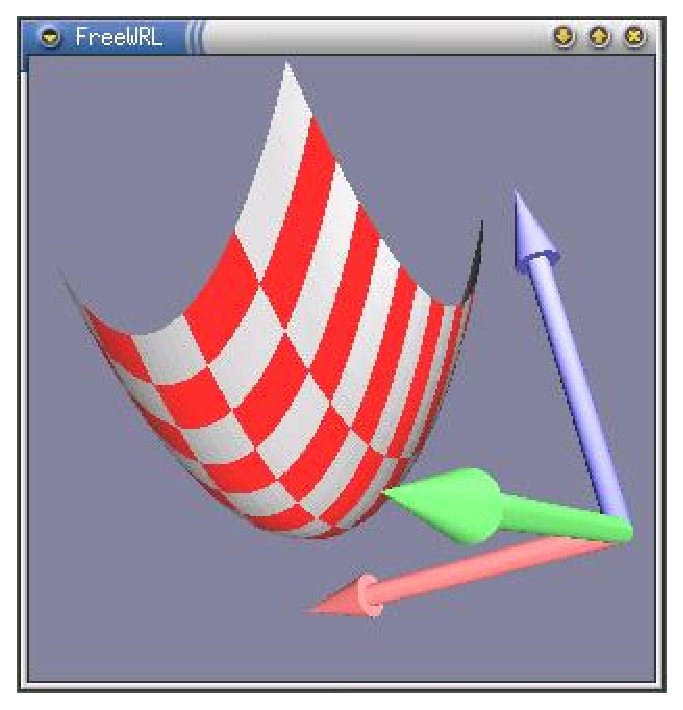
\includegraphics{figures/freewrl-checker-snap-3-c.eps}} ~\resizebox*{0.3\textwidth}{!}{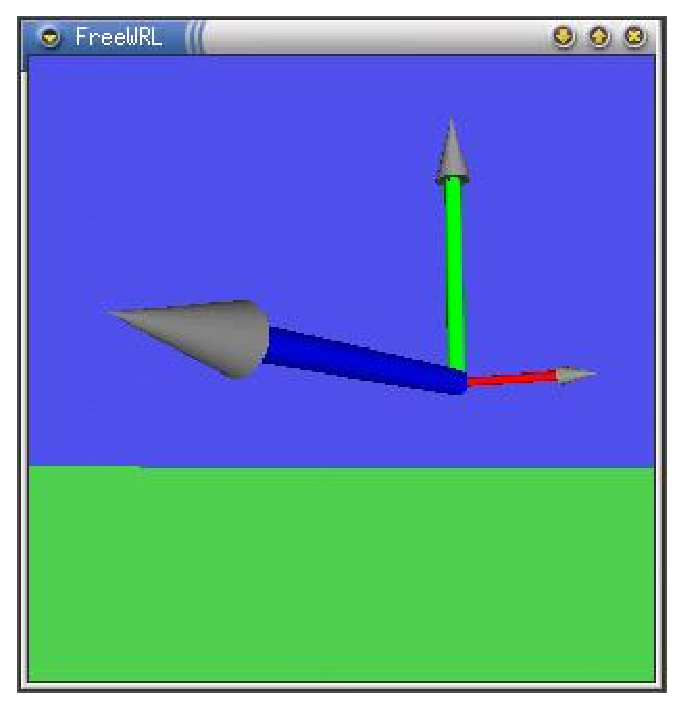
\includegraphics{figures/frame-sky-snap-c.eps}} ~\resizebox*{0.3\textwidth}{!}{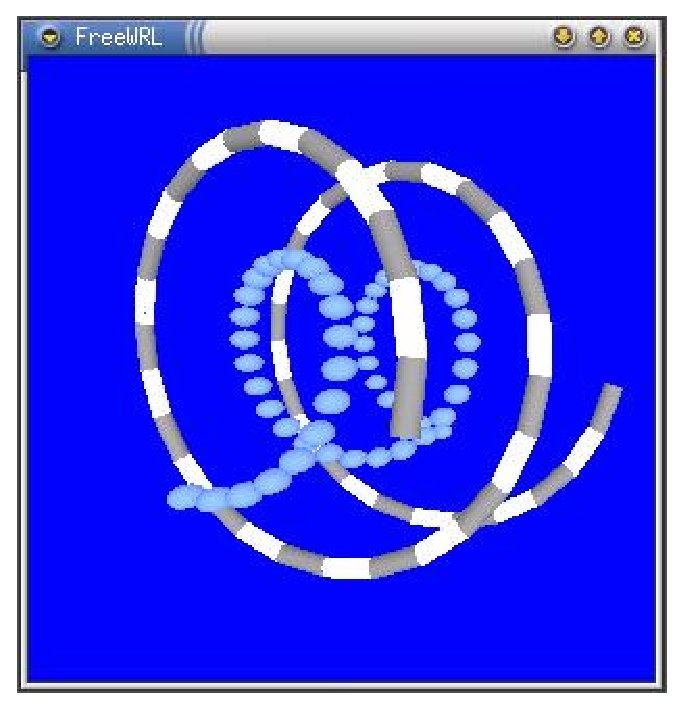
\includegraphics{figures/cyl-balls-snap-2-c.eps}} \par}


\caption{\textbf{\label{fig:misc}Left:} A checkered surface obtained by the
variant of Listing~1.\protect \\
\textbf{Middle:} An XYZ frame with axes colored red, blue and green,
obtained by running Listing~3.\protect \\
\textbf{Right:} A set of points connected by black and white cylinders
and the same set of points, scaled down by half along the Y and Z
axes (Listing~4).}
\end{figure}
The following listing and Figure~\ref{fig:misc}, middle, show an
example of the usage of \texttt{vrml\_frame()}, \texttt{vrml\_Background()},
and \texttt{vrml\_browse()}.


\subparagraph{Listing 3}

\begin{lyxcode}
s1~=~vrml\_frame~(\char`\"{}scale\char`\"{},{[}1~2~3{]},\char`\"{}col\char`\"{},eye~(3),~\char`\"{}hcol\char`\"{},0.5{*}{[}1~1~1{]});~\\
s2~=~vrml\_Background~(\char`\"{}skyColor\char`\"{},{[}3~3~9{]}/10,\char`\"{}groundColor\char`\"{},{[}3~8~3{]}/10);~\\
vrml\_browse~({[}s1,s2{]});
\end{lyxcode}
We now describe the function

\begin{description}
\item [\texttt{\textmd{s~=~vrml\_cyl~(x,...)}}]that returns VRML code
representing 3D \textbf{line segments} (in fact, cylinders) whose
extremities are \texttt{{[}x(:,i),x(:,i+1)}{]}, for \texttt{i} in
\( \left\{ 1,..,N\right\}  \) (\texttt{x} is a a \( 3\times N \)
matrix). Amongst other things, the radius, color and transparency
can be set. Also, spheres centered at each \texttt{x(:,i)} can be
added, and an arrow can be used to indicate the last segment. The
corresponding options are~:

\begin{description}
\item [\texttt{\textmd{\char`\"{}rad\char`\"{},~rad}}]The radius of the
cylinders linking each pair of consecutive points.
\item [\texttt{\textmd{\char`\"{}col\char`\"{},~col}}]\( 3\times 1 \)
or \( 3\times N \) The RGB color(s) of the cylinders.
\item [\texttt{\textmd{\char`\"{}tran\char`\"{},~col}}]The transparency
of the cylinders.
\item [\texttt{\textmd{\char`\"{}balls\char`\"{}}}]Add a spheres around
each \texttt{x(:,i)}.
\item [\texttt{\textmd{\char`\"{}arrow\char`\"{}}}]Represent the last segment
as an arrow.
\end{description}
\end{description}

\paragraph{Positioning, orienting and scaling objects}

Finally, we present a function that allows to translate, rotate and
scale an arbitrary VRML object and is useful for composing 3D setups
consisting of many object.

\begin{description}
\item [\texttt{\textmd{s~=~vrml\_transfo~(str,pos,rot,scale)}}]translates,
rotates and scales the object defined in the string \texttt{str}.
The arguments \texttt{pos} and \texttt{rot} represent a translation
and rotation respectively, just as in the \texttt{vrml\_frame()} function.
If \texttt{scale} is a scalar, the object \texttt{str} will be scaled
by that amount, while if \texttt{scale} is a \( 3\times 1 \) vector,
it represents the scaling of the X, Y and Z axes independently.
\end{description}
Listing~4 below and Figure~\ref{fig:misc} (right) illustrate how
the two functions introduced above can be used.


\subparagraph{Listing 4}

\begin{lyxcode}
x~=~linspace~(0,4{*}pi,50);

~~~~~~~~~~~~~~~~~~~~~~~~~~~\#~Points~on~a~helix

xx1~=~{[}x/6;~sin~(x);~cos~(x){]};



~~~~~~~~~~~~~~~~~~~~~~~~~~~\#~Linked~by~segments

s1~=~vrml\_cyl~(xx1,~\char`\"{}col\char`\"{},kron~(ones~(3,25),{[}0.7~0.3{]}));



~~~~~~~~~~~~~~~~~~~~~~~~~~~\#~Scaled~and~represented~by~spheres

s2~=~vrml\_points~(xx1,\char`\"{}balls\char`\"{});

s2~=~vrml\_transfo~(s2,nan,{[}pi/2,0,0{]},{[}1~0.5~0.5{]});

s3~=~vrml\_Background~(\char`\"{}skyColor\char`\"{},{[}0~0~1{]});

vrml\_browse~({[}s1,~s2,~s3{]});
\end{lyxcode}

\section{Summary and future plans\label{sec:conclusions}}

We have just passed in review the most important aspects of the VRML
toolbox. Its main utility is to examine surfaces and moderately sized
sets of points, but it can also be used to build and assemble more
general 3D objects.

The presented functionality is adapted to my personal needs; if you
think of some improvements, please send your suggestions (and perhaps
patches) to the mailing list \texttt{octave-dev@lists.sourceforge.net}.
In the future, I will focus on making more concise VRML code and articulating
better the library around that language.
\end{document}
